%-----------------------------------LICENSE------------------------------------%
%   This file is part of Mathematics-and-Physics.                              %
%                                                                              %
%   Mathematics-and-Physics is free software: you can redistribute it and/or   %
%   modify it it under the terms of the GNU General Public License as          %
%   published by the Free Software Foundation, either version 3 of the         %
%   License, or (at your option) any later version.                            %
%                                                                              %
%   Mathematics-and-Physics is distributed in the hope that it will be useful, %
%   but WITHOUT ANY WARRANTY; without even the implied warranty of             %
%   MERCHANTABILITY or FITNESS FOR A PARTICULAR PURPOSE.  See the              %
%   GNU General Public License for more details.                               %
%                                                                              %
%   You should have received a copy of the GNU General Public License along    %
%   with Mathematics-and-Physics.  If not, see <https://www.gnu.org/licenses/>.%
%------------------------------------------------------------------------------%

% Use the standalone class for displaying the tikz image on a small PDF.
\documentclass[crop, tikz]{standalone}

% Needed for mathbb.
\usepackage{amssymb}

% Import the tikz package to use for the drawing.
\usepackage{tikz}

% Load the arrows.meta library.
\usetikzlibrary{arrows.meta}

% Begin the document.
\begin{document}

    % Draw the figure.
    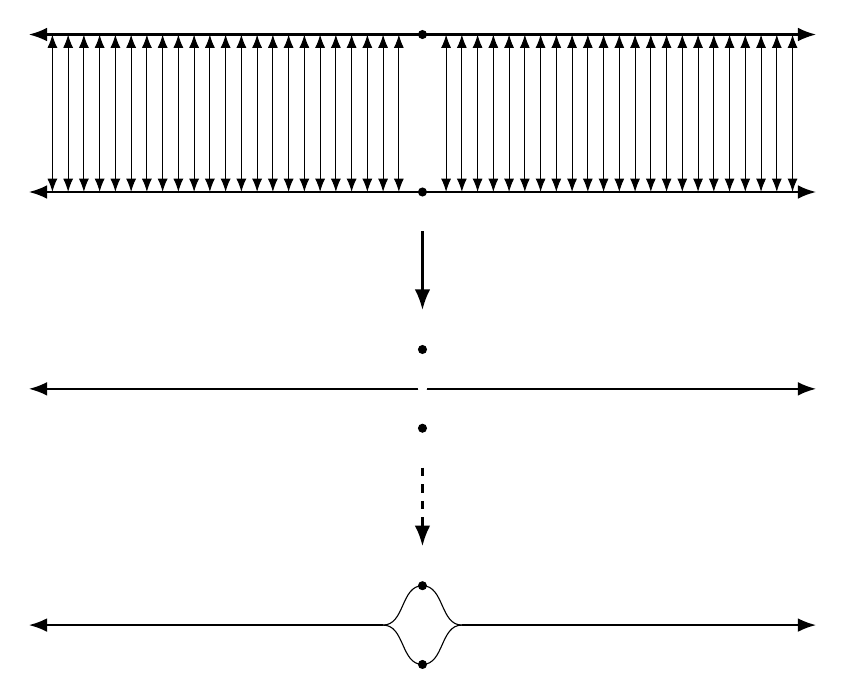
\begin{tikzpicture}[>=LaTeX]

        % Draw axes for the upper and lower lines (First figure).
        \draw[<->, thick] (-5, 0) to (5, 0);
        \draw[<->, thick] (-5, 2) to (5, 2);

        % Connect the dots for all points except for the two origins.
        \foreach\x in {-4.7, -4.5, ..., -0.3, 0.3, 0.5, ..., 4.7}{
            \draw[<->] (\x, 2) to (\x, 0);
        }

        % Fill in circles for the two origins.
        \draw[fill=black] (0, 0) circle (0.5mm);
        \draw[fill=black] (0, 2) circle (0.5mm);

        % Draw a solid arrow to the next graphic.
        \draw [->, line width=1pt] (0, -0.5) to (0, -1.5);

        % Draw the second figure shifted 2.5cm downwards.
        \begin{scope}[yshift=-2.5cm]
            % Draw the x-axis in the quotient space.
            \draw[<->, thick] (-5.0, 0.0) to (5.0, 0.0);

            % Remove the origin.
            \draw[fill=white, draw=white] (0, 0) circle (0.5mm);

            % Draw circles symbolizing the two origins.
            \draw[fill=black] (0.0,  0.5) circle (0.5mm);
            \draw[fill=black] (0.0, -0.5) circle (0.5mm);

            % Dashed arrow to the next graphic.
            \draw [->, line width=1pt, dashed] (0.0, -1.0) to (0.0, -2.0);
        \end{scope}

        % Draw the third figure shifted 5.5cm downwards.
        \begin{scope}[yshift=-5.5cm]
            % Draw the x-axis.
            \draw[<-, thick] (-5.0, 0.0) to (-0.5, 0);
            \draw[->, thick] ( 0.5, 0.0) to ( 5.0, 0);

            % Draw a curved line connecting the x-axis to the upper origin.
            \draw (-0.5, 0.0) to[out=0,in=180] (0.0, -0.5)
                              to[out=0,in=180] (0.5,  0.0);

            % Draw a curved line connecting the x-axis to the lower origin.
            \draw (-0.5, 0.0) to[out=0,in=180] (0.0, 0.5)
                              to[out=0,in=180] (0.5, 0.0);

            % Fill in the two origins.
            \draw[fill=black] (0.0,  0.5) circle (0.5mm);
            \draw[fill=black] (0.0, -0.5) circle (0.5mm);
        \end{scope}
    \end{tikzpicture}
\end{document}
